\section{Inequalities with $\ge$ and $>$}

\begin{tcbraster}[
    raster columns = 2,
    raster equal height,
    colback = white,
    ]
    \begin{tcolorbox}
        $|x| \ge 3$ 
        \tcblower
        \begin{center}
            \begin{tcolorbox}[center,colback=white,boxrule=0.5pt,]
                \small The distance of $x$ from the origin is \myEmph{greater than or equal to} $3$.
            \end{tcolorbox}
            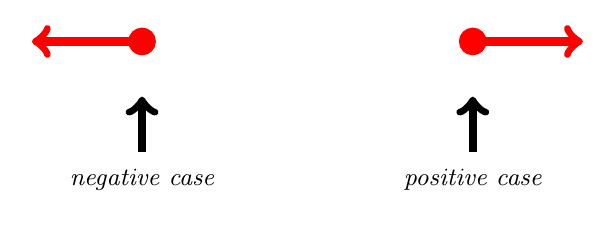
\begin{tikzpicture}[scale=0.7]
                \myDrawNumberlineCircle{0}{white}
                \whenTEACHER{
                    \draw [->,line width=3pt,red] (-3,0) -- (-5,0);
                    \draw[red,line width=3pt,fill=red] (-3,0) circle (0.175 cm);
                    %
                    \draw [->,line width=3pt,red] (3,0) -- (5,0);
                    \draw[red,line width=3pt,fill=red] (3,0) circle (0.175 cm);
                }
                \draw[->, black, line width=3pt] (-3,-2) -- (-3,-1);
                \node[] at (-3,-2.5) {\itshape\small negative case};
                \draw[->, black, line width=3pt] (3,-2)  -- (3,-1);
                \node[] at (3,-2.5) {\itshape\small positive case};
                \myDrawNumberline{5}
            \end{tikzpicture}\\
            \whenSTUDENT{\vspace{2\onelineskip}}
            %
            \whenTEACHER{
                {
                    $x \le -3$
                }
                \hfil
                {
                    $x \ge 3$
                }
            }
            \end{center}
    \end{tcolorbox}
    \begin{tcolorbox}
        $|x| > 3$ 
        \tcblower
        \begin{center}
            \begin{tcolorbox}[center,colback=white,boxrule=0.5pt,]
                \small The distance of $x$ from the origin is \myEmph{greater than} $3$.
            \end{tcolorbox}
            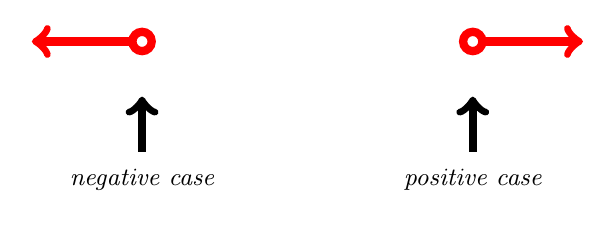
\begin{tikzpicture}[scale=0.7]
                \myDrawNumberlineCircle{0}{white}
                \whenTEACHER{
                    \draw [->,line width=3pt,red] (-3,0) -- (-5,0);
                    \draw[red,line width=3pt,fill=white] (-3,0) circle (0.175 cm);
                    %
                    \draw [->,line width=3pt,red] (3,0) -- (5,0);
                    \draw[red,line width=3pt,fill=white] (3,0) circle (0.175 cm);
                }
                \draw[->, black, line width=3pt] (-3,-2) -- (-3,-1);
                \node[] at (-3,-2.5) {\itshape\small negative case};
                \draw[->, black, line width=3pt] (3,-2)  -- (3,-1);
                \node[] at (3,-2.5) {\itshape\small positive case};
                \myDrawNumberline{5}
            \end{tikzpicture}\\
            \whenSTUDENT{\vspace{2\onelineskip}}
            %
            \whenTEACHER{
                {
                    $x < -3$
                }
                \hfil
                {
                    $x > 3$
                }
            }
            \end{center}
    \end{tcolorbox}
\end{tcbraster}

\begin{myConceptSteps}{To solve $|ax+b|\ge c$ or $|ax+b| > c$\dots}
    \myStep{check}{%
        If $c$ is \gap{negative}, 
        the solution is \gap{all} \gap{real} \gap{numbers}.
    }
    \myStep{two inequalities}{%
        Write \gap{two} inequalities:
            \begin{itemize}[nosep]
                \item $ ax+b$ \gap{$\le \text{\tiny or} <$} $-c$  
                \item $ ax+b$ \gap{$\ge \text{\tiny or} >$} $c$
            \end{itemize}
    }
    \myStep{solve}{Solve both inequalities.
    \begin{myWarningBox}[width=5.5in,center]
        \small\centering
        \gap{Multiplying}/\gap{dividing} by negatives \gap{flips} the inequality.
    \end{myWarningBox}
    }
    \myStep{result}{Write the result in two ways.
        \begin{itemize}[nosep]
            \item as two inequalities connected by \gap{OR}
            \item as two arrows on a number line
        \end{itemize}
    }
\end{myConceptSteps}

\myProblems[Solve these absolute value inequalities.]
{
    $|2x+1| > 5$
    \myAnswer{
        \hfill
        {\tiny 
            $x<-3$ OR $x>2$
        }
    }
}
{
    $|-2-3x| \ge 4$
    \myAnswer{
        \hfill
        {\tiny 
            $x\le-2$ OR $x\ge\frac{2}{3}$
        }
    }
}
{9\onelineskip}